\documentclass[tikz,border=2pt]{standalone}
\usepackage{newtxtext}
\usepackage{pgfplots}
\pgfplotsset{compat=1.18}
\usetikzlibrary{patterns}

\newcommand{\bparam}{b}
\newcommand{\cparam}{c}

\begin{document}
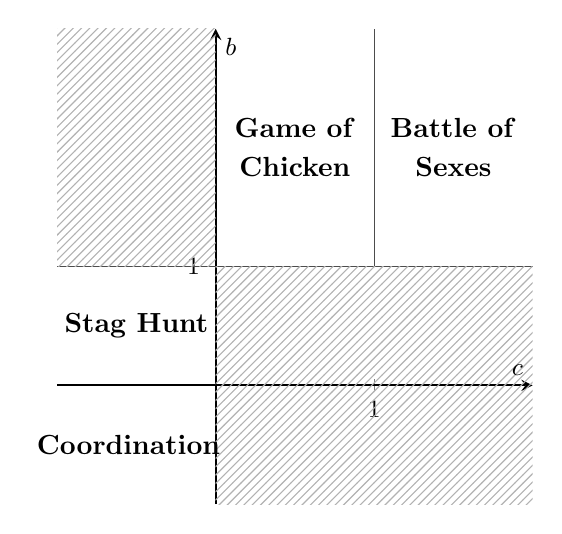
\begin{tikzpicture}
    \begin{axis}[
        width=3in,
        height=3in,
        axis x line=middle,
        axis y line=middle,
        axis line style={thick},
        xlabel={$\cparam$},
        ylabel={$\bparam$},
        xmin=-1, xmax=2,
        ymin=-1, ymax=3,
        xtick={0,1},
        ytick={0,1},
        tick label style={font=\small},
        label style={font=\small},
        enlargelimits=false,
        clip=false
    ]
    \addplot[black!70, thin] coordinates {(-1,1) (2,1)};
    \addplot[black!70, thin] coordinates {(1,1) (1,3)};
    \fill[pattern=north east lines, pattern color=gray!60]
         (axis cs:-1,1) -- (axis cs:0,1) -- (axis cs:0,3) -- (axis cs:-1,3) -- cycle;
    \fill[pattern=north east lines, pattern color=gray!60]
         (axis cs:2,1) -- (axis cs:0,1) -- (axis cs:0,-1) -- (axis cs:2,-1) -- cycle;
    \node at (axis cs:-0.5, 0.5) {\normalsize \textbf{Stag Hunt}};
    \node at (axis cs:-0.55,-0.5) {\normalsize \textbf{Coordination}};
    \node[align=center] at (axis cs:1.5,2) {\normalsize \textbf{Battle of}\\[2pt]\normalsize \textbf{Sexes}};
    \node[align=center] at (axis cs:0.5,2) {\normalsize \textbf{Game of}\\[2pt]\normalsize \textbf{Chicken}};
    \end{axis}
\end{tikzpicture}
\end{document}
